\section{\Large{Лекция 3}}

\begin{wrapfigure}{H}{0.5\linewidth}
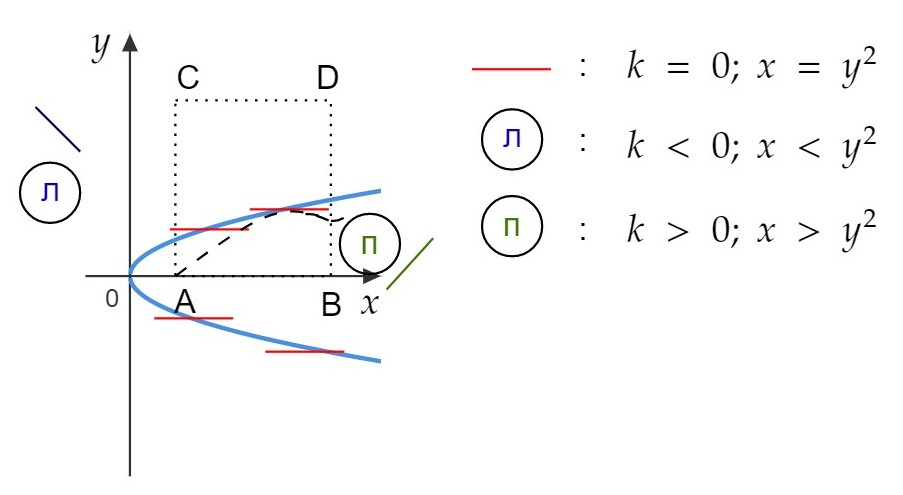
\includegraphics[width=\linewidth]{images/p4.jpg}
\caption[]{}
\label{ris2}
\end{wrapfigure}
\begin{example}
    Доказать: решение $y = \varphi(x)$, $x \in (a,b)$ задачи Коши
    \begin{equation*}
        \begin{cases}
        y' = x - y^2, 
        \\
        y(1) = 0
        \end{cases}
    \end{equation*}
    
    можно продолжить на интервал $(a, +\infty)$.
    
    \begin{enumerate}
        \item $f(x,y) = x - y^2$ --- непр.
        
        $f_y = -2y$ --- непр.
        
        Значит, существует единственное решение в некоторой $\delta$-окрестности точки 1  задачи Коши по теореме о существовании и единственности.
        
        \item Точка $(1,0) \in G$, для этого нужно, чтобы $x_0\in(a,b)$
        
        \item Нам на пути еще не раз встретятся уравнения Риккати:
        
        \begin{equation*}
            \cfrac{dy}{dx} = P(x)y^2 + Q(x)y + R(x)
        \end{equation*}
        --- в общем виде оно не интегрируемо в квадратурах. В некоторых случаях решение можно найти аналитически. Наше --- не из таких. Нужно воспользоваться:
            \begin{enumerate} 
            \item Качественным анализом поведения интегральных кривых (метод изоклин)
            \item Теоремой о продолжении решения до границы ограниченной области.
             \end{enumerate}
    \end{enumerate}   
    
    Зафиксируем $f(x,y) = x - y^2 = 0$: на кривой $x = y^2$ изоклины параллельны оси абсцисс. (см. Рис. \ref{ris2})
    
    Возьмем точки: A(1,0), B($b^2$, 0), $b > 1$, C(1, 2$b$), D($b^2, 2b$). ABCD --- область $G$. По теореме о продолжении решения до границы, интегральная кривая, выходящая из (1,0) (пунктир) попадет на BD, не выйдет из области. Так как $b$ мы брали произвольное, решение можно продолжить на (1, $\infty$).
\end{example}

\begin{theorem}  \fcolorbox{o}{o}{О продолжении решения на весь заданный интервал.}

Пусть: \begin{itemize}
    \item $G = \{\alpha < x < \beta, y \in \R\}$. Допускается, что $\alpha = -\infty$ или $\beta = +\infty$.
    \item $f(x,y) \in C(G), f'_y\in C(G)$. ($y' = f(x,y)$)
    \item $\exists a(x) \in C(\alpha,\beta)$, $\exists b(x) \in C(\alpha,\beta)$, причем $a(x) \geqslant 0$, $b(x) \geqslant 0$.
    \item Выполнена оценка: $\big|f(x,y)\big| \leqslant a(x)|y(x)| + b(x)$ $\forall x \in (\alpha,\beta)$
\end{itemize}

тогда любое решение ОДУ(\ref{2.2}), проходящее в области $G$, можно продолжить на весь интервал $(\alpha,\beta)$.
\end{theorem}

Доказательство будет на Новый год $\Smiley$

\begin{example}\label{ex3.1}
    Доказать: задача Коши
    \begin{equation}
        \begin{cases}
        y' = y+2-\sin y \\
        y(0) = 0
        \end{cases}
    \end{equation} имеет решение, определенное на всей вещественной оси.
\end{example}

\subsection{\large{ОДУ 1-го порядка, приводимые к ДУ с разделяющимися переменными}}

\subsubsection{Уравнение вида}
\begin{equation*}
    y' = f(ax+by+c)
\end{equation*}
\begin{prop}
    приводится к ОДУ с РП заменой $z(x) = ax+by(x)+c.$
\end{prop}

Действительно, тогда $z' = a+by'$, $y' = \cfrac{z'-a}{b}$. Получаем уравнение такого вида:

$z' - a = bf(z)$, или $z' = a + bf(z) = g(z)$.
\vspace{3mm}
\begin{example}  $y' = \cos(y-x)$

    Замена: $z(x) = y (x) - x$
    
    $z' = y' - 1 \Rightarrow z'+1 = \cos z$
    
    Получаем уравнение $z' = \cos z - 1$, теперь переменные легко разделяются.
    \begin{enumerate}
        \item $\cfrac{dz}{\cos z - 1} = dx$, $\cos z\neq 1$.
        
        $\displaystyle \int \cfrac{dz}{-2\sin^2\frac{z}{2}} = \int dx$
        
        $\ctg \cfrac{z}{2} = x + c$
        
        $\ctg \cfrac{y-x}{2} = x+c$
        \item $\cos z = 1$
        
        $z = 2 \pi k, k \in \Z$
        
        Уравнение становится таким: $\cfrac{dz}{dx} = 0$. $\cos z - 1 = 0$, значит, это решение.
    \end{enumerate}
    Ответ: $y = x +2\arctg(x+c)$, $y = x + 2 \pi k$, $k \in \Z$.
\end{example}

\subsubsection{Геометрические свойства семейств интегральных кривых.}

\textbf{Рассмотрим уравнение 3.1.2(а):}
\begin{equation}\label{3.1.2(а)}
    \cfrac{dy}{dx} = f(x)
\end{equation}

При замене $\Tilde{x} = x$, $\Tilde{y} = y+c$, $c = const$  уравнение не изменит вид. В таких случаях говорят: уравнение является инвариантным относительно замены переменных.

Если $\Phi(x,y) = 0$ --- интеграл (частный), а

$\Phi(\Tilde{x}, \Tilde{y}) = 0$ --- тоже интеграл, получаем 

$\Phi(x, y+c) = 0$ $\forall c \in \R$ --- общий интеграл.

Итак, зная частный интеграл, можно найти общий интеграл.

Уравнение \ref{3.1.2} допускает параллельный перенос интегральных кривых вдоль оси $OY$. При этом линии $x = x_0$ --- изоклины: $f(x_0) = const$.

\begin{Def} Множество преобразований \fcolorbox{g}{g}{образует группу}, если:
    \begin{enumerate}
        \item Есть тождественный элемент (переходит в себя)
        \item Для любого преобразования существет обратное
        \item Произведение (композиция) преобразований тоже принадлежит этому множеству.
    \end{enumerate}
\end{Def}

$\Rightarrow$ параллельный перенос --- группа.

\textbf{Рассмотрим уравнение 3.1.2(б):}
\begin{equation}\label{3.1.2(б)}
    \cfrac{dy}{dx}=f(y)
\end{equation}

Замена: $\Tilde{x} = x + c$, $\Tilde{y} = y$ --- параллельный перенос вдоль $OX$. Тоже образует группу преобразований.

Если знаем частный интеграл $\Phi(x,y) = 0$, то знаем и общий интеграл $\Phi(x+c, y) = 0$.

$y = y_0$ --- изоклины: $f(y_0) = const$.

\subsubsection{ОДУ с однородной правой частью}

\begin{Def}
    Фуекция одного или нескольких переменных $f(x_1, \ldots, x_n)$ называется \fcolorbox{g}{g}{однородной степени $k$}, если существует число $k$: $\forall \lambda$ $f(x_1,\ldots,x_n) = \lambda^kf(x_1,\ldots, x_n)$.
    
    Указанное число $k$ --- \fcolorbox{g}{g}{степень (показатель) однородности}.
\end{Def}

\begin{Def}
    ОДУ 1-го порядка в форме Коши $\cfrac{dy}{dx} = f(x,y)$ называется \fcolorbox{g}{g}{однородным относительно $x$ и $y$}, если $f(x,y)$ является однородной функцией своих переменных с показателем однородности равным 0.
\end{Def}

Пусть $y' = f(x,y)$ --- однородное.

Возьмём $\lambda = \frac{1}{x}$: $f\brackets{\frac{1}{x}x, \frac{1}{x}y} = f\brackets{1, \frac{y}{x}} = \Tilde{f}\brackets{\frac{y}{x}}$

\textbf{ОДУ вида $y' = f\brackets{\frac{x}{y}}$ --- однородное.}  \label{3.3.1}

Относительно каких преобразований оно инвариантно?

\textbf{Рассмотрим группу преобразований} $\Tilde(x) = cx$, $\Tilde{y} = cy$ (гомотетия).

Изоклины: $f\brackets{\frac{x}{y}} = const$.

Если $\Phi(x,y) = 0$ --- частный интеграл, то $\Phi(cx, cy) = 0$ --- общий интеграл.

\begin{prop} \fcolorbox{o}{o}{Лейбница}
    Замена $z(x) = \cfrac{y(x)}{x}$ приводит однородное ОДУ $y' = f\brackets{\frac{x}{y}}$  ОДУ с РП.
\end{prop}

Покажем это. $y(x) = x\cdot z(x)$

$f\brackets{\frac{x}{y}} = y' = z + xz' = f(z)$

или $xz' = f(z) - z = \Tilde{f}(z)$. Тут переменные разделяются.

\subsubsection{ОДУ, приводимые к однородным или с разделяющимися переменными}

\begin{prop}
    ОДУ вида
    \begin{equation}\label{3.4.1}
        \cfrac{dy}{dx}= f\brackets{\cfrac{a_1x+b_1y+c_1}{a_2x+b_2y+c_2}}
    \end{equation} приводится к ОДУ с разделяющимися переменными.
\end{prop}

Рассмотрим два случая.
\vspace{5mm}

1) $c_1 = c_2 = 0$

Однородная $f\brackets{\cfrac{a_1x+b_1y}{a_2x+b_2y}} = f\brackets{\cfrac{a_1+b_1\frac{y}{x}}{a_2+b_2\frac{y}{x}}} = \Tilde{f}\brackets{\cfrac{y}{x}}$ --- однородная с показателем однородности $k = 0$.
\vspace{3mm}

2) $c_1^2+c_2^2 \neq 0$,
$\begin{vmatrix}
  a_1& b_1\\
  a_2& b_2
\end{vmatrix} \neq 0$

Тогда система уравнений  \begin{equation*}
        \begin{cases}
        a_1x+b_1y+c_1=0
        \\
        a_2x+b_2y+c_2=0
        \end{cases}
    \end{equation*} задает две пересекающиеся прямые, существует единственное решение $x = \alpha, \ y = \beta$.
    
Перенесем начало координат в точку пересечения прямых:

$\Tilde{x}=x - \alpha$, $\Tilde{y} = y - \beta$.

$\Tilde{dx} = dx$, $\Tilde{dy} = dy$.

Получим уравнение: 

\begin{eqnarray} \cfrac{dy}{dx} = \cfrac{\Tilde{dy}}{\Tilde{dx}} = f\brackets{\cfrac{a_1(\Tilde{x}+\alpha)+b_1(\Tilde{y}+\beta)+c_1}{a_2(\Tilde{x}+\alpha)+b_2(\Tilde{y}+\beta)+c_2}} = f\brackets{\cfrac{a_1\Tilde{x}+b_1\Tilde{y}+[a_1\alpha+b_1\beta+c_1]}{a_2\Tilde{x}+b_2\Tilde{y}+[a_2\alpha+b_2\beta+c_2]}} = \\
 = f\brackets{\cfrac{a_1\Tilde{x}+b_1\Tilde{y}}{a_2\Tilde{x}+b_2\Tilde{y}}}
\end{eqnarray}
 

Теперь возвращаемся к пункту 1): уравнение приводится к РП.
\vspace{3mm}

3) $\begin{vmatrix}
  a_1& b_1\\
  a_2& b_2
\end{vmatrix} = 0$. Тогда $a_1=\gamma a_2$, $b_1 = \gamma b_2$.

$\cfrac{dy}{dx} = f\brackets{\cfrac{\gamma a_2 x + \gamma b_2 y + \gamma c_2 + c_1 - \gamma c_2}{a_2 x + b_2 y + c_2}} = g\brackets{a_2x+b_2y+c_2}$

Такое уже встречалось. Знаем, что надо делать замену $z(x) = a_2x+b_2y+c_2$.